\message{ !name(msm-manual.Rnw.tex)}
\message{ !name(msm-manual.Rnw) !offset(838) }
\section{Fitting multi-state models with {\tt msm}}

<<echo=FALSE>>=
options(width = 60)
@

\Rpackage{msm} is a package of functions for multi-state modelling using
the R statistical software.  The \Rfunction{msm} function itself
implements maximum-likelihood estimation for general multi-state
Markov or hidden Markov models in continuous time. We illustrate
its use with a set of data from monitoring heart transplant patients.
Throughout this section ``\textsl{\texttt{>}}'' indicates the R
command prompt, \textsl{\texttt{slanted typewriter}} text indicates R
commands, and \texttt{typewriter} text R output.

\subsection{Installing \tt{msm}}
\label{sec:installing}

The easiest way to install the \Rpackage{msm} package on a computer
connected to the Internet is to run the R command:

\begin{Scode}
  install.packages("msm")
\end{Scode}

This downloads \Rpackage{msm} from the CRAN archive of contributed R
packages (\texttt{cran.r-project.org} or one of its mirrors) and
installs it to the default R system library.  To install to a
different location, for example if you are a normal user with no
administrative privileges, create a directory in which R packages are
to be stored, say, \texttt{/your/library/dir}, and run

\begin{Scode}
  install.packages("msm", lib='/your/library/dir')
\end{Scode}

After \Rpackage{msm} has been installed, its functions can be made
visible in an R session by
<<>>=
library(msm)
@
or, if it has been installed into a non-default library,

\begin{Scode}
  library(msm, lib.loc='/your/library/dir')
\end{Scode}


\subsection{Getting the data in}
\label{sec:datain}

The data are specified as a series of observations, grouped by
patient. At minimum there should be a data frame with variables
indicating
\begin{itemize}
\item the time of the observation,
\item the observed state of the process.
\end{itemize}
If the data do not also contain
\begin{itemize}
\item the subject identification number,
\end{itemize}
then all the observations are assumed to be from the same subject.
The subject ID does not need to be numeric, but data must be grouped
by subject, and observations must be ordered by time within subjects.
If the model includes variables with missing values, then the corresponding
observations  are omitted by \Rfunction{msm} with a warning.  If you have missing data,
as in any statistical model, it is recommended to ensure these do not
result in biases.

An example data set, taken from monitoring a set of heart transplant
recipients, is provided with \Rpackage{msm}.  (Note: since \Rpackage{msm}
version 1.3, the command \Rfunction{data(cav)} is no longer needed to
load the data --- it is now ``lazy-loaded'' when required). Sharples
\etal \cite{my:cav} studied the progression of coronary allograft
vasculopathy (CAV), a post-transplant deterioration of the arterial
walls, using these data.  Risk factors and the accuracy of the
screening test were investigated using multi-state Markov and hidden
Markov models.

The first three patient histories are shown below. There are 622
patients in all.  \Robject{PTNUM} is the subject identifier.
Approximately each year after transplant, each patient has an
angiogram, at which CAV can be diagnosed.  The result of the test is
in the variable \Robject{state}, with possible values 1, 2, 3
representing CAV-free, mild CAV and moderate or severe CAV
respectively.  A value of 4 is recorded at the date of death.
\Robject{years} gives the time of the test in years since the heart
transplant. Other variables include \Robject{age} (age at screen),
\Robject{dage} (donor age), \Robject{sex} (0=male, 1=female),
\Robject{pdiag} (primary diagnosis, or reason for transplant - IHD
represents ischaemic heart disease, IDC represents idiopathic dilated
cardiomyopathy), \Robject{cumrej} (cumulative number of rejection
episodes), and \Robject{firstobs}, an indicator which is 1 when the
observation corresponds to the patient's transplant (the first
observation), and 0 when the observation corresponds to a later
angiogram.

<<>>=
cav[1:21,]
@

A useful way to summarise multi-state data is as a frequency table of
pairs of consecutive states.  This counts over all individuals, for
each state $r$ and $s$, the number of times an individual had an
observation of state $r$ followed by an observation of state $s$. The
function \Rfunction{statetable.msm} can be used to produce such a table,
as follows,

<<>>=
statetable.msm(state, PTNUM, data=cav)
@
Thus there were 148 CAV-free deaths, 48 deaths from state 2, and
55 deaths from state 3.  On only four occasions was there an
observation of severe CAV followed by an observation of no CAV.   


\subsection{Specifying a model}
\label{sec:specifying:model}

We now specify the multi-state model to be fitted to the data.  A
model is governed by a transition intensity matrix $Q$. For the heart
transplant example, there are four possible states through which the
patient can move, corresponding to CAV-free, mild/moderate CAV, severe
CAV and death.  We assume that the patient can advance or recover from
consecutive states while alive, and die from any state. Thus the model
is illustrated by Figure \ref{fig:disease} with four states, and we
have

\[
Q = \left(
  \begin{array}{llll}
    -(q_{12} + q_{14}) & q_{12} &  0     & q_{14}\\
    q_{21} & -(q_{21}+q_{23}+q_{24}) & q_{23} & q_{24}\\
      0    & q_{32} & -(q_{32}+q_{34}) & q_{34}\\
      0    &   0    &   0    &   0   \\
  \end{array}
\right )
\]

It is important to remember that this defines which
\emph{instantaneous} transitions can occur in the Markov process, and
that the data are \emph{snapshots} of the process (see
section \ref{sec:arbitr-observ-times}).  Although there were 44
occasions on which a patient was observed in state 1 followed by state
3, we can still have $q_{13}=0$. The underlying model specifies that the patient must have passed
through state 2 in between, rather than jumping straight from 1 to 3.  If your data represent the exact and
complete transition times of the process, then you must specify
\Rfunarg{exacttimes=TRUE} or \Rfunarg{obstype=2} in the call to
\Rfunction{msm}.

To tell \Rfunction{msm} what the allowed transitions of our model are,
we define a matrix of the same size as $Q$, containing zeroes in the
positions where the entries of $Q$ are zero.  All other positions
contain an initial value for the corresponding transition intensity.
The diagonal entries supplied in this matrix do not matter, as the
diagonal entries of $Q$ are defined as minus the sum of all the other
entries in the row.  This matrix will eventually be used as the
\Rfunarg{qmatrix} argument to the \Rfunction{msm} function. For
example,

<<>>=
Q  <-  rbind ( c(0, 0.25, 0, 0.25),
               c(0.166, 0, 0.166, 0.166),
               c(0, 0.25, 0, 0.25),
               c(0, 0, 0, 0) )
@

Fitting the model is a process of finding values of the seven unknown
transition intensities: $q_{12}$, $q_{14}$, $q_{21}$, $q_{23}$,
$q_{24}$, $q_{32}$, $q_{34}$, which maximise the likelihood.

\subsection{Specifying initial values}
\label{sec:inits}

The likelihood is maximised by numerical methods, which need a set of
initial values to start the search for the maximum.  For reassurance
that the true maximum likelihood estimates have been found, models
should be run repeatedly starting from different initial
values. However a sensible choice of initial values can be important
for unstable models with flat or multi-modal likelihoods.  For
example, the transition rates for a model with misclassification could
be initialised at the corresponding estimates for an approximating
model without misclassification. Initial values for a model without
misclassification could be set by supposing that transitions between
states take place only at the observation times.  If we observe
$n_{rs}$ transitions from state $r$ to state $s$, and a total of $n_r$
transitions from state $r$, then $q_{rs} / q_{rr}$ can be estimated by
$n_{rs} / n_r$. Then, given a total of $T_r$ years spent in state $r$,
the mean sojourn time $1 / q_{rr}$ can be estimated as $T_r / n_r$.
Thus, $n_{rs} / T_r$ is a crude estimate of $q_{rs}$.

Such default initial values can be used by supplying
\Rfunarg{gen.inits=TRUE} in the call to \Rfunction{msm} below, along
with a \Rfunarg{qmatrix} whose non-zero entries represent the allowed
transitions of the model.  Alternatively the function \Rfunction{crudeinits.msm}
could be used to get this matrix of initial values explicitly as follows.
These methods are only available for non-hidden Markov models.

<<>>=
Q.crude  <- crudeinits.msm(state ~ years, PTNUM, data=cav,
                                   qmatrix=Q)
@

However, if there are are many changes of state in between the
observation times, then this crude approach may fail to give sensible
initial values.  For the heart transplant example we could also guess
that the mean period in each state before moving to the next is about
2 years, and there is an equal probability of progression, recovery or
death.  This gives $q_{rr} = - 0.5$ for $r = 1, 2, 3$, and $q_{12} =
q_{14} = 0.25$, $q_{21} = q_{23} = q_{24} = 0.166$, $q_{32} = q_{34} =
0.25$, and the initial value matrix \Robject{Q} shown above,
which we now use to fit the model.

\subsection{Running \Rfunction{msm}}
\label{sec:running}

To fit the model, call the \Rfunction{msm} function with the appropriate
arguments.  For our running example, we have defined a data set
\Robject{cav}, a matrix \Robject{Q} indicating the allowed
transitions, and initial values. We are ready to run \Rfunction{msm}.

\paragraph{Model 1: simple bidirectional model}


<<>>=
cav.msm <- msm( state ~ years, subject=PTNUM, data = cav,
                    qmatrix = Q, deathexact = 4)
@

In this example the day of death is assumed to be recorded exactly, as
is usual in studies of chronic diseases.  At the previous instant
before death the state of the patient is unknown.  Thus we specify
\Rfunarg{deathexact = 4}, to indicate to \Rfunction{msm} that the
entry times into state 4 are observed in this manner.
If the model had
five states, and states 4 and 5 were two competing causes of death with
times recorded exactly in this way, then we would specify \Rfunarg{deathexact =
  c(4,5)}.

By default, the data are assumed to represent snapshots of the process
at arbitrary times.  However, observations can also represent exact
times of transition, ``exact death times'', or a mixture of these. See the
\Rfunarg{obstype} argument to \Rfunction{msm}.  

While the \Rfunction{msm} function runs, it searches for the maximum
of the likelihood of the unknown parameters.  Internally, it uses the
R function \Rfunction{optim} to minimise the minus log-likelihood.
When the data set, the model, or both, are large, then this may take a
long time.  It can then be useful to see the progress of the
optimisation algorithm. To do this, we can specify a \Rfunarg{control}
argument to \Rfunction{msm}, which is passed internally to the
\Rfunction{optim} function.  For example \texttt{control = list(trace=1,
  REPORT=1)}. See the help page for \Rfunction{optim},

<<eval=FALSE>>=
help(optim)
@
for more options to control the optimisation. \footnote{Note that since version 1.3.2, \Rfunarg{method=''BFGS''}, is the default optimisation algorithm in \Rfunction{msm}, since it can use analytic derivatives, which are available for most models.}

When completed, the \Rfunction{msm} function returns a value.  This
value is a list of the important results of the model fitting,
including the parameter estimates and their covariances.  To keep
these results for post-processing, we store them in an R object, here
called \Robject{cav.msm}.  When running several similar
\Rfunction{msm} models, it is recommended to store the respective
results in informatively-named objects.


\subsection{Showing results}

To show the maximum likelihood estimates and 95\% confidence
intervals, type the name of the fitted model object at the R command
prompt.  \footnote{This is equivalent to typing
  \texttt{print.msm(cav.msm)}.  The function \Rfunction{print.msm}
  formats the important information in the model object for printing
  on the screen.}  The confidence level can be changed using the
\Rfunarg{cl} argument to \Rfunction{msm}.

<<>>=
cav.msm
@

From the estimated intensities, we see patients are three times
as likely to develop symptoms than die without symptoms (transitions from state 1).
After disease onset (state 2), progression to severe symptoms (state
3) is 50\% more likely than recovery.  Once in the severe state, death
is more likely than recovery, and a mean of 1 / -0.44 = 2.3 years is
spent in state 3 before death or recovery.

Section \ref{sec:extractor} describes various functions that can be
used to obtain summary information from the fitted model.


\subsection{Covariates on the transition rates}
\label{sec:msm:covariates}

We now model the effect of explanatory variables on the rates of
transition, using a proportional intensities model. Now we have an
intensity matrix $Q(z)$ which depends on a covariate vector $z$. For
each entry of $Q(z)$, the transition intensity for patient $i$ at
observation time $j$ is $q_{rs}(z_{ij}) = q_{rs}^{(0)}
\exp(\beta_{rs}^T z_{ij})$.  The covariates $z$ are specified through
the \Rfunarg{covariates} argument to \Rfunction{msm}. If $z_{ij}$ is
time-dependent, we assume it is constant in between the observation
times of the Markov process.  \Rfunction{msm} calculates the
probability for a state transition from times $t_{i,j-1}$ to $t_{ij}$
using the covariate value at time $t_{i,j-1}$.

We consider a model with just one covariate, female sex.  Out of the
622 transplant recipients, 535 are male and 87 are female.  By
default, all linear covariate effects $\beta_{rs}$ are initialised to
zero. To specify different initial values, use a \Rfunarg{covinits}
argument, as described in \Rfunction{help(msm)}.  Initial values given
in the \Rfunarg{qmatrix} represent the intensities with covariate values
set to their means in the data.  In the following model, all transition
intensities are modelled in terms of sex.

\paragraph{Model 2: sex as a covariate}
<<>>=
cavsex.msm <- msm( state ~ years, subject=PTNUM, data = cav,
                     qmatrix = Q, deathexact = 4, covariates = ~ sex)
@

Printing the \Robject{msm} object now displays the estimated covariate
effects and their confidence intervals (note since version 1.3.2 these
are \emph{hazard ratios} $\exp(\beta_{rs})$, not \emph{log hazard ratios} $\beta_{rs}$ as in previous
versions).

<<>>=
cavsex.msm
@
The sizes of the
confidence intervals for some of the hazard ratios suggests there is no information in the data about 
the corresponding covariate effects, leading to a likelihood that is a flat function of these parameters, 
and this model should be simplified. The first column shown in the output
is the estimated transition intensity matrix
$q_{rs}(z) = q_{rs}^{(0)} \exp(\beta_{rs}^T z)$ with the covariate $z$
set to its mean value in the data.  This represents an average
intensity matrix for the population of 535 male and 87 female
patients. To extract separate intensity matrices for male and female
patients ($z = 0$ and $1$ respectively), use the function
\Rfunction{qmatrix.msm}, as shown below.  This and similar summary
functions will be described in more detail in
section \ref{sec:extractor}.

<<>>=
qmatrix.msm(cavsex.msm, covariates=list(sex=0)) # Male
qmatrix.msm(cavsex.msm, covariates=list(sex=1)) # Female
@

Since \Rpackage{msm} version 1.2.3, different transition rates may be
easily modelled on different covariates by specifying a named list of
formulae as the \Rfunarg{covariates} argument.  Each element of the
list has a name identifying the transition.  In the model below, the
transition rate from state 1 to state 2 and the rate from state 1 to
state 4 are each modelled on sex as a covariate, but no other
intensities have covariates on them.

\paragraph{Model 2a: transition-specific covariates}
<<eval=FALSE>>=
cavsex.msm <- msm( state ~ years, subject=PTNUM, data = cav,
                  qmatrix = Q, deathexact = 4,
                  covariates = list("1-2" = ~ sex, "1-4" = ~sex) )
@

We may also want to constrain the effect of a covariate to be equal for
certain transition rates, to reduce the number of parameters in the
model, or to investigate hypotheses on the covariate effects.  A
\Rfunarg{constraint} argument can be used to indicate which of the
transition rates have common covariate effects.

\paragraph{Model 3: constrained covariate effects}

<<eval=FALSE>>=
cav3.msm <- msm( state ~ years, subject=PTNUM, data = cav,
                qmatrix = Q, deathexact = 4,
                covariates = ~ sex,
                constraint = list(sex=c(1,2,3,1,2,3,2)) )
@

This constrains the effect of sex to be equal for the progression
rates $q_{12}, q_{23}$, equal for the death rates $q_{14}, q_{24},
q_{34}$, and equal for the recovery rates $q_{21}, q_{32}$. The
intensity parameters are assumed to be ordered by reading across the
rows of the transition matrix, starting at the first row: ($q_{12},
q_{14}, q_{21}, q_{23}, q_{24}, q_{32}, q_{34}$), giving constraint
indicators \Rfunarg{(1,2,3,1,2,3,2)}.  Any vector of increasing
numbers can be used for the indicators.  Negative entries can be used
to indicate that some effects are equal to minus others:
\Rfunarg{(1,2,3,-1,2,3,2)} sets the fourth effect to be minus the
first.

In a similar manner, we can constrain some of the baseline transition
intensities to be equal to one another, using the
\Rfunarg{qconstraint} argument.  For example, to constrain the rates
$q_{12}$ and $q_{23}$ to be equal, and $q_{24}$ and $q_{34}$ to be
equal, specify \Rfunarg{qconstraint = c(1,2,3,1,4,5,4)}.



\subsection{Fixing parameters at their initial values}

For exploratory purposes we may want to fit a model assuming that some
parameters are fixed, and estimate the remaining parameters.  This may
be necessary in cases where there is not enough information in the
data to be able to estimate a proposed model, and we have strong prior
information about a certain transition rate. To do this, use the
\Rfunarg{fixedpars} argument to \Rfunction{msm}.  For model 1, the
following statement fixes the parameters numbered 6, 7, that is,
$q_{32}$, $q_{34}$, to their initial values (0.25 and 0.25,
respectively).

\paragraph{Model 4: fixed parameters}
<<eval=FALSE>>=
cav4.msm <- msm( state ~ years, subject=PTNUM, data = cav,
                qmatrix = Q, deathexact = 4,
                control = list(trace=2, REPORT=1),
                fixedpars = c(6, 7) )
@

A \Rfunarg{fixedpars} statement can also be used for fixing covariate
effect parameters to zero, that is to assume no effect of a covariate
on a certain transition rate.

\subsection{Extractor functions}
\label{sec:extractor}

We may want to extract some of the information from the \Rfunction{msm}
model fit for post-processing, for example for plotting graphs or
generating summary tables.  A set of functions is provided for
extracting interesting features of the fitted model.

\begin{description}

\item[Intensity matrices] The function \Rfunction{qmatrix.msm}
  extracts the estimated transition intensity matrix and its confidence intervals
  for a given set of covariate values, as shown in
  section \ref{sec:msm:covariates}.  Confidence intervals are
  calculated from the covariance matrix of the estimates by assuming
  the distribution is symmetric on the log scale.  Standard errors for
  the intensities are also available from the object returned by
  \Rfunction{qmatrix.msm}.  These are calculated by the delta method.
  The \Rpackage{msm} package provides a general-purpose function
  \Rfunction{deltamethod} for estimating the variance of a function of
  a random variable $X$ given the expectation and variance of $X$. See
  \texttt{help(deltamethod)} for further details.  Bootstrap
  confidence intervals are also available for \Rfunction{qmatrix.msm}
  and for most output functions; these are often more accurate, at the
  cost of computational time.  For more about bootstrapping in
  \Rpackage{msm}, see Section \ref{sec:boot}.

\item[Transition probability matrices] The function
  \Rfunction{pmatrix.msm} extracts the estimated transition probability
  matrix $P(t)$ within a given time. For example, for model 1, the 10
  year transition probabilities are given by:

<<>>=
pmatrix.msm(cav.msm, t=10)
@

  Thus, a typical person in state 1, disease-free, has a probability
  of 0.5 of being dead ten years from now, a probability of 0.3 being
  still disease-free, and probabilities of 0.1 of being alive with
  mild/moderate or severe disease, respectively.

  This assumes $Q$ is constant within the desired time interval.  For
  non-homogeneous processes, where $Q$ varies with time-dependent
  covariates but can be approximated as piecewise constant, there is
  an equivalent function \Rfunction{pmatrix.piecewise.msm}.  Consult its
  help page for further details.

  If \Rfunarg{ci=''norm''} is specified, then a confidence interval is
  calculated based on drawing a random sample (default size 1000) from
  the assumed multivariate normal distribution of the maximum
  likelihood estimates and covariance matrix, and transforming.  If
  \Rfunarg{ci=''boot''} is specified, then a bootstrap confidence
  interval for the transition probability matrix is calculated (see Section \ref{sec:boot}) .
  However, both of these are computationally intensive, particularly
  the bootstrap method, so no confidence interval is calculated by default.

\item[Mean sojourn times] The function \Rfunction{sojourn.msm}
  extracts the estimated mean sojourn times in each transient state
  $r$, for a given set of covariate values. This is calculated as $-1
  / \hat q_{rr}$, where $\hat q_{rr}$ is the $r$th diagonal entry of
  the estimated transition intensity matrix.

<<>>=
sojourn.msm(cav.msm)
@

\item[Probability that each state is next] The function
  \Rfunction{pnext.msm} extracts the matrix of probabilities $-q_{rs}
  / q_{rr}$ that the next state after state $r$ is state $s$, for each
  $r$ and $s$.  Together with the mean sojourn times, this gives a more
  intuitive parameterisation of a continuous-time Markov model than
  the raw transition intensities $q_{rs}$.  Note these are different from
  the transition probabilities in a given time $t$ returned by
  \Rfunction{pmatrix.msm}.

<<>>=
pnext.msm(cav.msm)
@

\item[Total length of stay] Mean sojourn times describe the
  average period in a single stay in a state. For processes with
  successive periods of recovery and relapse, we may want to
  forecast the total time spent healthy or diseased, before
        death.  The function \Rfunction{totlos.msm} estimates the
        forecasted total length of time spent in each transient state
        $s$ between two future time points $t_1$ and $t_2$, for a
        given set of covariate values. This defaults to the expected
        amount of time spent in each state between the start of the
        process (time 0, the present time) and death or a specified
        future time. This is obtained as
\[
L_s = \int_{t_1}^{t_2} P(t)_{r,s} dt
\]
where $r$ is the state at the start of the process, which defaults to
1. This is calculated using numerical integration.  For model 1, each
patient is forecasted to spend 8.8 years disease free, 2.2 years with
mild or moderate disease and 1.8 years with severe disease.

Bootstrap and asymptotic confidence intervals are available, as for
\Rfunction{pmatrix.msm}, but are not calculated by default.

<<>>=
totlos.msm(cav.msm)
@

\item[Expected first passage times] The function \Rfunction{efpt.msm} estimates
  the expected time until the process first enters a given state or set of states,
  also called the ``hitting time''.  See its help page for further details.

\item[Expected number of visits] The function \Rfunction{envisits.msm}
  estimates the expected number of visits to a state, computed in a
  similar way to the total length of stay. See its help page for
  further details.

\item[Ratio of transition intensities] The function
  \Rfunction{qratio.msm} estimates a ratio of two entries of the
  transition intensity matrix at a given set of covariate values,
  together with a confidence interval estimated assuming normality on
  the log scale and using the delta method.  For example, we may want
  to estimate the ratio of the progression rate $q_{12}$ into the
  first state of disease to the corresponding recovery rate $q_{21}$.
  For example in model 1, recovery is 1.8 times as likely as
  progression.

<<>>=
qratio.msm(cav.msm, ind1=c(2,1), ind2=c(1,2))
@

\item[Hazard ratios for transition] The function \Rfunction{hazard.msm}
  gives the estimated hazard ratios corresponding to each covariate
  effect on the transition intensities. 95\% confidence limits are
  computed by assuming normality of the log-effect.

<<>>=
hazard.msm(cavsex.msm)
@

\end{description}

\paragraph{Setting covariate values}
All of these extractor functions take an argument called
\Rfunarg{covariates}.  If this argument is omitted, for example,

<<eval=FALSE>>=
qmatrix.msm(cav.msm)
@
then the intensity matrix is evaluated as $Q(\bar x)$ with all
covariates set to their mean values $\bar x$ in the data.
Alternatively, set \Rfunarg{covariates} to 0 to return the result
$Q(0)$ with covariates set to zero. This will usually be
preferable for categorical covariates, where we wish to see the
result for the baseline category.

<<eval=FALSE>>=
qmatrix.msm(cavsex.msm, covariates = 0)
@
Alternatively, the desired covariate values can be specified
explicitly as a list,

<<eval=FALSE>>=
qmatrix.msm(cavsex.msm, covariates = list(sex = 1))
@

Values of categorical covariates must be quoted. For example, consider
a covariate \texttt{smoke}, representing tobacco smoking status, with
three levels, \texttt{NON, CURRENT, EX}, representing a non-smoker,
current smoker or ex-smoker.

\begin{Scode}
qmatrix.msm(example.msm, covariates = list(age = 60, smoke=''CURRENT''))
\end{Scode}


\subsection{Survival plots}

In studies of chronic disease, an important use of multi-state models
is in predicting the probability of survival for patients in
increasingly severe states of disease, for some time $t$ in the
future.  This can be obtained directly from the transition probability
matrix $P(t)$.

The \Rfunction{plot} method for \Robject{msm} objects produces a plot
of the expected probability of survival against time, from each
transient state. Survival is defined as not entering the final
absorbing state.

<<fig=TRUE>>=
plot(cav.msm, legend.pos=c(8, 1))
@

This shows that the 10-year survival probability with severe CAV is
approximately 0.1, as opposed to 0.3 with mild CAV and 0.5 without
CAV.  With severe CAV the survival probability diminishes very quickly
to around 0.3 in the first five years after transplant.  The
\Rfunarg{legend.pos} argument adjusts the position of the legend in
case of clashes with the plot lines.  A \Rfunarg{times} argument can
be supplied to indicate the time interval to forecast survival for.

A more sophisticated analysis of these data might explore competing
causes of death from causes related or unrelated to the disease under
study.

\subsection{Bootstrapping}
\label{sec:boot}
Most of \Rpackage{msm}'s output functions present confidence intervals
based on asymptotic standard errors calculated from the Hessian, or
transformations of these using the delta method.  The asymptotic
standard errors are expected to be underestimates of the true standard
errors (Cramer-Rao lower bound).  For some output functions, such as
\Rfunction{pmatrix.msm}, and functions based on
\Rfunction{pmatrix.msm} such as \Rfunction{totlos.msm} and
\Rfunction{prevalence.msm}, the delta method cannot be used at all to
obtain standard errors.  In these cases, confidence intervals can be
calculated by drawing a random sample from the assumed multivariate
normal distribution of the maximum likelihood estimates and covariance
matrix, and transforming.  However, this is still based on potentially
inaccurate asymptotic theory.  The \Rpackage{msm} package provides the
function \Rfunction{boot.msm} to enable bootstrap refitting of
\Rfunction{msm} models, an alternative way to estimate uncertainty.

For non-hidden Markov models, a bootstrap dataset is drawn by
resampling pairs of consecutive states from the full data, i.e.
\emph{transitions}.  These are assumed to be independent when
calculating the likelihood (Section \ref{sec:multi:likelihood}).  For
hidden Markov models and models with censoring, a bootstrap dataset is
drawn by resampling complete series from independent subjects.  The
bootstrap datasets have the same number of transitions, or subjects,
respectively, as the original data.

For most output extractor functions provided with \Rpackage{msm}, the
option \Rfunarg{ci=''boot''} is available, as a wrapper around
\Rfunction{boot.msm}, to enable bootstrap confidence intervals to be calculated.
But any user-defined output statistic can be bootstrapped, as follows.
The function \Rfunction{boot.msm} is called with the fitted
\Rfunction{msm} model as first argument, and an R function specifying
the statistic to be bootstrapped as the second argument \texttt{stat}.
The return value from \Rfunction{boot.msm} is a list of \texttt{B}
replicates (by default, \texttt{B=1000}) of the desired statistic.  For
example, to bootstrap the transition intensity matrix of the heart
transplantation model \Robject{cav.msm}:
\begin{Scode}
  q.list <- boot.msm(cav.msm, stat=function(x){qmatrix.msm(x)$estimates})
\end{Scode}
Note that for \Rfunction{boot.msm} to be able to refit the original
model that produced \Robject{cav.msm}, all objects used in the
original model fit (for example, in this case, \Robject{Q})
must be in the working environment.  Otherwise, \Rfunction{boot.msm}
will give an ``object not found'' error.

The user can then summarise these replicates by calculating empirical
standard deviations or quantile-based intervals.  In this example,
\Robject{q.list} is a list of 1000 4$\times$4 matrices.  The following
code calculates the bootstrap standard error as the empirical standard
deviation of the 1000 replicates, and a similar 95\% bootstrap
confidence interval.
\begin{Scode}
  q.array <- array(unlist(q.list), dim=c(4,4,1000))
  apply(q.array, c(1,2), sd)
  apply(q.array, c(1,2), function(x)quantile(x, c(0.025, 0.975)))
\end{Scode}

Note that when bootstrapping, the refits of the model to the resampled
datasets may occasionally fail to converge (as discussed in
Section \ref{sec:failure}) even if the original model fit did
converge.  In these cases, a warning is given, but
\Rfunction{boot.msm} simply discards the failed dataset and moves on
to the next bootstrap iteration. Unless convergence failure occurs for
a large proportion of iterations, this should not affect the accuracy
of the final bootstrap confidence intervals.


\subsection{Convergence failure}
\label{sec:failure}

Inevitably if over-complex models are applied with insufficient data
then the parameters of the model will not be identifiable.  This will
result in the optimisation algorithm failing to find the maximum of
the log-likelihood, or even failing to evaluate the likelihood. For
example, it will commonly be inadvisable to include several covariates
in a model simultaneously.

In some circumstances, the optimisation may report convergence, but
fail to calculate any standard errors.  In these cases, the Hessian of
the log-likelihood at the reported solution is not positive definite.
Thus the reported solution may be a saddle point rather than the
maximum likelihood, or it may be close to the maximum.

\begin{description}

\item[Model simplification]

  Firstly, make sure there are not too many parameters in the model.  There may not be enough
  information in the data on a certain transition rate.  It is
  recommended to count all the pairs of transitions between states in
  successive observation times, making a frequency table of previous
  state against current state (function \Rfunction{statetable.msm}),
  and do this for any subgroups defining covariates.
  Although the data are a series of snapshots of a continuous-time
  process, and the actual transitions take place in between the
  observation times, this type of table may still be helpful.  If
  there are not many observed `transitions' from state 2 to state 4,
  for example, then the data may be insufficient to estimate $q_{24}$.

  For a staged disease model (Figure \ref{fig:disease}), the number of
  disease states should be low enough that all transition rates can be
  estimated.  Consecutive states of disease severity should be merged
  if necessary.  If it is realistic, consider applying constraints on
  the intensities or the covariate effects so that the parameters are
  equal for certain transitions, or zero for certain transitions.

  Be careful to use a observation scheme and transition matrix
  appropriate to your data (see
  Section \ref{sec:arbitr-observ-times}). By default, \Rfunction{msm}
  assumes that the data represent snapshots of the process, and the
  true state is unknown between observation times.  In such
  circumstances, it is rarely feasible to estimate an intensity matrix
  with \emph{instantaneous} transitions allowed between every pair of
  states.  This would be easier if the complete course of the process
  is known \Rfunarg{(exacttimes = TRUE)} in the call to
  \Rfunction{msm}.  Understand the difference between
  \emph{instantaneous} and \emph{interval} transitions - although
  individuals may be in state 1 at time $t_r$, and state 3 at time
  $t_{r+1}$, that doesn't mean that instantaneous transitions from 1
  to 3 should be permitted.


\item[Initial values] Make sure that a sensible set of initial values
  have been chosen. The optimisation may only converge within a
  limited range of `informative' initial values.  It is also sensible
  to run the model for several different initial values to ensure that
  the estimation has converged to a global rather than a local optimum.

\item[Scaling] It is often necessary to apply a scaling factor to normalise the likelihood (\Rfunarg{fnscale}), or certain individual parameters \Rfunarg{(parscale)}.  This may prevent overflow or underflow problems within the optimisation.  For example, if the value of the -2 $\times$ log-likelihood is around 5000, then the following option leads to an minimisation of the -2 $\times$ log-likelihood on an approximate unit scale: \Rfunarg{control = list(fnscale = 5000)}.  
  % Though since version 1.4.1, \Rfunarg{fnscale} is applied automatically using the likelihood at the initial values, unless the user has already supplied it.
%    If not provided by the user, \code{control=list(fnscale = a)} is
%    applied automatically to normalise the optimisation, where \code{a}
%    is the minus twice log likelihood at the initial values.

  It is also advisable to analyse all variables, including covariates
  and the time unit, on a roughly normalised scale. For example,
  working in terms of a time unit of months or years instead of days,
  when the data range over thousands of days.

\item[Convergence criteria] ``False convergence'', in which
  \Rfunction{optim()} reports convergence of the optimisation but the
  Hessian is not positive definite, can sometimes be solved by
  tightening the criteria (\Rfunarg{reltol}, defaults to
  \texttt{1e-08}) for reporting convergence. For example,
  \Rfunarg{control = list(reltol = 1e-16)}.

  Alternatively consider using smaller step sizes for the numerical
  approximation to the gradient, used in calculating the Hessian.
  This is given by the control parameter \Rfunarg{ndeps}. For example,
  for a model with 5 parameters, \Rfunarg{control = list(ndeps =
    rep(1e-6, 5))}

\item[Choice of algorithm] By default, since version 1.3.2,
  \Rfunction{msm} uses the BFGS method of \Rfunction{optim}, which
  makes use of analytic derivatives.  Analytic derivatives are
  available for all models in msm, apart from hidden Markov models
  with unknown initial state probabilities, misclassification models
  with equality constraints on misclassification probabilities, and
  truncated or measurement-error outcome distributions.  This speeds
  up optimisation.  Though alternative algorithms are available such
  as \Rfunarg{method = ``CG''}.  Or use the \Rfunction{nlm} R function
  via \Rfunarg{msm(..., opt.method = "nlm" , ...)}  Note also the
  Fisher scoring method available for non-hidden Markov models for
  panel data, via \Rfunarg{msm(..., opt.method = "fisher", ...)}, is
  expected to be faster than the generic methods, but less robust to
  bad initial values.  Or since version 1.3.2, msm can also use
  \Rfunarg{method=``bobyqa''} from the \Rpackage{minqa} package, a fast
  derivative-free method.

\item[\Rfunction{optim} "function cannot be evaluated at initial parameters"]
  To diagnose this problem, run \Rfunction{msm} again with
  \Rfunarg{fixedpars=TRUE} set, to calculate the -2 log-likelihood at
  the initial values.  This will probably be \Robject{Inf}. To show
  the contributions of individual subjects to the overall log
  likelihood, call \Rfunction{logLik.msm(x, by.subject=TRUE)}, where
  \Robject{x} is the fitted model object.  If only a few subjects give
  an infinite log-likelihood, then you can check whether their state
  histories are particularly unusual and conflict with the model.  For
  example, they might appear to make unusually large jumps between
  states in short periods of time.  For models with misclassification,
  note that the default true initial state distribution
  \Rfunarg{initprobs} puts all individuals in true state 1 at their
  first observation.  If someone starts in a much higher state, this
  may result in an infinite log-likelihood, and changing
  \Rfunarg{initprobs} would be sensible.


\end{description}


\subsection{Model assessment}
\label{sec:model-assessment}

\paragraph{Observed and expected prevalence}

To compare the relative fit of two nested models, it is easy to
compare their likelihoods.  However it is not always easy to determine
how well a fitted multi-state model describes an irregularly-observed
process.  Ideally we would like to compare observed data with fitted
or expected data under the model.  If there were times at which all
individuals were observed then the fit of the expected numbers in each
state or {\em prevalences} can be assessed directly at those times.
Otherwise, some approximations are necessary.  We could assume that an
individual's state at an arbitrary time $t$ was the same as the state
at their previous observation time.  This might be fairly accurate if
observation times are close together.  This approach is taken by the
function \Rfunction{prevalence.msm}, which constructs a table of observed
and expected numbers and percentages of individuals in each state at a
set of times.

A set of expected counts can be produced if the process begins at a
common time for all individuals.  Suppose at this time, each
individual is in state 0.  Then given $n(t)$ individuals are under
observation at time $t$, the expected number of individuals in state
$r$ at time $t$ is $n(t) P(t)_{0,r}$.   If the covariates on which
$P(t)$ depends vary between individuals, then this can be
averaged over the covariates observed in the data.

For example, we calculate the observed and expected numbers and
percentages at two-yearly intervals up to 20 years after transplant,
for the heart transplant model \Rfunction{cav.msm}.  The number of
individuals still alive and under observation decreases from 622 to
251 at year 20.  The observed and expected percentages are plotted
against time.

<<>>=
options(digits=3)
prevalence.msm(cav.msm, times=seq(0,20,2))
@
<<fig=TRUE>>=
plot.prevalence.msm(cav.msm, mintime=0, maxtime=20)
@

Comparing the observed and expected percentages in each state,
we see that the predicted number of individuals who die (State 4) is
under-estimated by the model from about year 8 onwards.  Similarly the
number of individuals sill alive and free of CAV (State 1) is
over-estimated by the model from about year 8 onwards.

Such discrepancies could have many causes.  One possibility is that
the transition rates vary with the time since the beginning of the
process, the age of the patient, or some other omitted covariate, so
that the Markov model is {\em non-homogeneous}.  This could be
accounted for by modelling the intensity as a function of age, for
example, such as a piecewise-constant function.  The \Rfunarg{pci}
argument to \Rfunction{msm} can be used to automatically construct
models with transition intensities which are piecewise-constant in
time.

In this example, the hazard of death may increase with age, so that
the model underestimates the number of deaths when forecasting far
into the future.  Another cause of poor model fit may sometimes be the
failure of the Markov assumption.  That is, the transition intensities
may depend on the time spent in the current state (a semi-Markov
process) or other characteristics of the process history.  Accounting
for the process history is difficult as the process is only observed
through a series of snapshots.  Semi-Markov 
models may in principle be fitted to this type of data using phase-type distributions.  Since
version 1.4.1 the \Rfunarg{phase.states} option to \Rfunction{msm} can be used to 
define some phase-type models.  See \Rfunction{help(msm)} for further details.

However, if it is known that individuals who died would not have been
followed up after a certain time, had they survived to that time, then
they should not be included in the observed prevalence of the death
state after that time.  This can be accounted for by passing a vector
of maximum potential follow-up times, one for each individual in the
same order as the original data, in the \Rfunarg{censtime} argument to
\Rfunction{prevalence.msm}.  Ignoring the potential follow-up times is
likely to have resulted in overestimates of the number of deaths
at later times in the CAV example, though these times are not
available in the data supplied with \Rpackage{msm}.


\paragraph{Pearson-type goodness-of-fit test}
\label{sec:pearson}

Suppose that the true transition times are unknown, and data consist
of observations of the process at arbitrary times which differ between
individuals (panel data).  Assessing goodness of fit by prevalence
counts then involves estimating the observed prevalence at a series of
points by some form of interpolation. This is only advisable if
observation times are close together.  An alternative method of
assessing goodness-of-fit is to construct tables of observed and
expected numbers of transitions, as described by Aguirre-Hernandez and
Farewell \cite{ahf}.  This leads to a formal test of goodness-of-fit,
analogous to the classical Pearson $\chi^2$ test for contingency
tables. The tables are constructed as follows.  Each pair of
successive observations in the data (\emph{transition}) is classified
by
\begin{itemize}
\item the starting state $r$ and finishing state $s$,
\item time between the start of the process and the first of the pair
  of observations (indexed by $h$),
\item time interval between the observations (indexed by $l_h$, within
  categories $h$),
\item (if there are fitted covariates) the impact of covariates, as
  summarised by $q_{rr}$ (indexed by $c$),
\item any other grouping of interest for diagnosing lack of fit
  (indexed by $g$).
\end{itemize}
Groupings of continuous quantities are normally defined by quantiles,
so that there are a similar number of observed transitions in each
(one-dimensional) category.  The observed and expected numbers of
transitions in each group are then defined by
\[
o_{hl_h rscg} = \sum I(S(t_{i,j+1}) = s, S(t_{ij}) = r)
\]
\[
e_{hl_h rscg} = \sum P(S(t_{i,j+1}) = s | S(t_{ij}) = r)
\]
where $I(A)$ is the indicator function for an event $A$ and the
summation is over the set of transitions in the category defined by
$h,l_h,c,g$, over all individuals $i$. The Pearson-type test statistic
is then
\[
T = \sum_{hl_h rscg} \frac{(o_{hl_h rscg} - e_{hl_h rscg})^2}{e_{hl_h rscg}}
\]
The classical Pearson test statistic is distributed as $\chi^2_{n-p}$,
where $n$ is the number of independent cells in the table and $p$ is
the number of estimated parameters $p$. But the null distribution of
$T$ is not exactly $\chi^2$, since the time intervals are
non-identical, therefore the observed transitions are realizations
from a set of independent but non-identical multinomial distributions.
Titman \cite{titman:asympnull} showed that the null distribution
of $T$ is asymptotically approximated by a weighted sum of $\chi^2_1$
random variables.   Aguirre-Hernandez and Farewell \cite{ahf} also showed that $\chi^2_{n-p}$
is a good approximation if there are no fitted covariates. For models
with covariates, the null mean of $T$ is higher than $n - p$, but
lower than $n$.  Therefore, upper and lower bounds for the true
$p$-value of the statistic can be obtained from the $\chi^2_{n-p}$ and
$\chi^2_n$ distributions.  Aguirre-Hernandez and Farewell \cite{ahf}
also described a bootstrap procedure for obtaining an accurate $p$-value.

Titman and Sharples \cite{titman:sharples} described modifications to
the test to correct for the biases introduced where in addition to the
panel-data observation scheme:
\begin{itemize}
\item Times of death are known exactly.  In this case, transitions
  ending in death are classified according to the next scheduled
  observation time after the death, which is estimated by multiple
  imputation from a Kaplan-Meier estimate of the distribution of time
  intervals between observations.

\item An individual's final observation is censored, so that they are
  only known to be alive at that point.

\item States are misclassified.
\end{itemize}

The \Rpackage{msm} package provides the function
\Rfunction{pearson.msm} to perform the Pearson-type test.  By default,
three groups are used for each of $h$, $l_h$ and $c$.  Often the
number of groups will need to be reduced in cases where the resulting
contingency tables are sparse (thus there are several low expected
counts and the variance of $T$ is inflated).

The test is now performed on the model \Robject{cav.msm} for the heart
transplant dataset (a version of which was also analysed by
Titman and Sharples \cite{titman:sharples}). The default three interval groups are used,
and two groups of the time since the start of the process. The
\Rfunarg{transitions} argument groups the transitions from state 3 to
each of states 1, 2 and 3 (the 9th, 10th and 11th transitions)
together in the table, since these transitions are infrequent.

<<>>=
options(digits=2)
pearson.msm(cav.msm, timegroups=2,
            transitions=c(1,2,3,4,5,6,7,8,9,9,9,10))
@

The first two tables in the output show the contingency tables of
observed and expected numbers of transitions.  Note that the observed
number of transitions in certain categories is not a whole number,
since these are averaged over multiple imputations of the next
scheduled observation time following deaths.  The column \texttt{Time}
is the group defined by time since the start of the process, and the
column \texttt{Interval} is the group defined by intervals between
observations.  The columns indicate the allowed transitions, or pairs
of states which can be observed in successive observations.

The third table presents the ``deviance'', the value of
$\frac{(o_{hl_h rscg} - e_{hl_h rscg})^2}{e_{hl_h rscg}}$ for each
cell, multipled by the sign of $o_{hl_h rscg} - e_{hl_h rscg}$ to
indicate whether there were more or fewer transitions than expected in
each cell.  These can indicate areas of bad fit.  For example,
systematic changes in deviance by time or time interval between
observations can indicate that a model with time-varying transition
intensities is more suitable.  Changes in deviance by covariate impact
may indicate heterogeneity between individuals which is unexplained
by the fitted covariates.  Changes in deviance with the length of the
interval between observations may also indicate failure of the Markov
assumption, and that a semi-Markov model (in which intensities depend
on the time spent in the current state) may fit better.

In this example, the test statistic is 100.  \Robject{p.upper} is an
upper bound for the $p$-value of the statistic based on an asymptotic
$\chi^2_{42}$ distribution, therefore the model does not fit well.  It
is not clear from the table of deviances which aspects of the fit are
most influental to the test statistic.  However, the two-way Markov
model itself is not biologically plausible, as discussed in
Section \ref{sec:fitting:hmm:misc}.

For non-hidden Markov models for panel data, \Rfunction{pearson.msm}
also presents the accurate analytic p-value of
Titman \cite{titman:asympnull}.  For all models,
\Rfunction{pearson.msm} provides an option for parametric
bootstrapping to obtain an accurate p-value.


\subsection{Fitting misclassification models with \Rpackage{msm}}
\label{sec:fitting:hmm:misc}

In fact, in the heart transplant example from
section \ref{sec:datain}, it is not medically realistic for patients
to recover from a diseased state to a healthy state.  Progression of
coronary artery vasculopathy is thought to be an irreversible process.
The angiography scan for CAV is actually subject to error, which leads
to some false measurements of CAV states and apparent recoveries.
Thus we account for misclassification by fitting a \emph{hidden Markov
model} using \Rpackage{msm}.  Firstly we replace the two-way multi-state
model by a one-way model with transition intensity matrix
\[
Q = \left(
  \begin{array}{llll}
    -(q_{12} + q_{14}) & q_{12} &  0     & q_{14}\\
      0    & -(q_{23}+q_{24}) & q_{23} & q_{24}\\
      0    &   0    & -q_{34} & q_{34}\\
      0    &   0    &   0    &   0   \\
  \end{array}
\right )
\]
We also assume that true state 1 (CAV-free) can be classified as state
1 or 2, state 2 (mild/moderate CAV) can be classified as state 1, 2 or
3, while state 3 (severe CAV) can be classified as state 2 or 3.
Recall that state 4 represents death.  Thus our matrix of misclassification
probabilities is
\[
E = \left(
  \begin{array}{llll}
    1 - e_{12} & e_{12} & 0 & 0 \\
    e_{21} & 1 - e_{21} - e_{23} & e_{23} & 0 \\
    0 & e_{32} & 1 - e_{32} & 0 \\
    0 & 0 & 0 & 0\\
  \end{array}
  \right)
\]
with underlying states as rows, and observed states as columns.

To model observed states with misclassification, we define a matrix
\Rfunarg{ematrix} indicating the states that can be misclassified.
Rows of this matrix correspond to true states, columns to observed
states.  It should contains zeroes in the positions where
misclassification is not permitted.  Non-zero entries are initial
values for the corresponding misclassification probabilities. We then
call \Rfunction{msm} as before, but with this matrix as the
\Rfunarg{ematrix} argument.  Initial values of 0.1 are assumed for
each of the four misclassification probabilities $e_{12}, e_{21},
e_{23}, e_{32}$.  Zeroes are given where the elements of $E$ are zero.
The diagonal elements supplied in \Rfunarg{ematrix} are ignored, as
rows must sum to one. The matrix \Rfunarg{qmatrix}, specifying
permitted transition intensities and their initial values, also
changes to correspond to the new $Q$ representing the progression-only
model for the underlying states.

The true state for every patient at the date of transplant is known to
be ``CAV-free'', not misclassified.  To indicate this we use the
argument \Rfunarg{obstrue} to \Rfunction{msm}.  This is set to be a
variable in the dataset, \Rfunarg{firstobs}, indicating where the
observed state equals the true state.  This takes the value of 1 at
the patient's first observation, at the transplant date, and 0
elsewhere.

We use an alternative quasi-Newton optimisation algorithm
\Rfunarg{(method="BFGS")} which can often be faster or more robust
than the default Nelder-Mead simplex-based algorithm.  An optional
argument \Rfunarg{initprobs} could also have been given here,
representing the vector of the probabilities of occupying each true
state at the initial observation
(equation \ref{eq:multi:hidden:matprod}).  This can also be a matrix
with number of rows equal to the number of subjects, if these
probabilities are subject-dependent and known. If not given, all
individuals are assumed to be in true state 1 at their initial
observation.  If \Rfunarg{est.initprobs=TRUE} is specified, then these
probabilites are estimated as part of the model fit, using
a vector \Rfunarg{initprobs} as initial values.  Covariate effects on these
probabilities can also be estimated using a multinomial logistic
regression model, if an \Rfunarg{initcovariates} argument is
specified.  See \Rfunction{help(msm)} for further details.


\paragraph{Model 5: multi-state model with misclassification}

<<>>=
Qm <- rbind(c(0, 0.148, 0, 0.0171),
            c(0, 0, 0.202, 0.081),
            c(0, 0, 0, 0.126),
            c(0, 0, 0, 0))
ematrix <- rbind(c(0, 0.1, 0, 0),
                 c(0.1, 0, 0.1, 0),
                 c(0, 0.1, 0, 0),
                 c(0, 0, 0, 0))
cavmisc.msm <- msm(state ~ years, subject = PTNUM, data = cav,
                   qmatrix = Qm, ematrix = ematrix, deathexact = 4,
                   obstrue = firstobs)
cavmisc.msm
@

Thus there is an estimated probability of about 0.03 that
mild/moderate CAV will be diagnosed erroneously, but a rather higher
probability of 0.17 that underlying mild/moderate CAV will be
diagnosed as CAV-free.  Between the two CAV states, the mild state
will be misdiagnosed as severe with a probability of 0.06, and the
severe state will be misdiagnosed as mild with a probability of 0.12.

The model also estimates the progression rates through underlying
states.  An average of 8 years is spent disease-free, an average of
about 3 years is spent with mild/moderate disease, and periods of severe
disease also last about 3 years on average before death.

\subsection{Effects of covariates on misclassification rates}

We can investigate how the probabilities of misclassification depend
on covariates in a similar way to the transition intensities, using a
\Rfunarg{misccovariates} argument to \Rfunction{msm}. For example, we
now include female sex as a covariate for the misclassification
probabilities.  The linear effects on the log odds of each misclassified
state relative to the true state are initialised to zero by default (but
this can be changed with the \Rfunarg{misccovinits} argument).


\paragraph{Model 6: misclassification model with misclassification probabilities modelled on sex}

<<>>=
cavmiscsex.msm <- msm(state ~ years, subject = PTNUM, data = cav,
                      qmatrix = Qm, ematrix = ematrix,
                      deathexact = 4, misccovariates = ~sex,
                      obstrue=firstobs)
@
<<>>=
cavmiscsex.msm
@
The large confidence interval for the odds ratio for 1/2 misclassification suggests
there is no information in the data about the difference between genders in 
the false positive rates for angiography. On the other hand, women have slightly more
false negatives.


\subsection{Extractor functions}

As well as the functions described in section \ref{sec:extractor} for
extracting useful information from fitted models, there are a number
of extractor functions specific to models with misclassification.

\begin{description}
\item[Misclassification matrix] The function \Rfunction{ematrix.msm}
gives the estimated misclassification probability matrix at the given
covariate values.  For illustration, the fitted misclassification
probabilities for men and women in model 6 are given by

<<>>=
ematrix.msm(cavmiscsex.msm, covariates=list(sex=0))
ematrix.msm(cavmiscsex.msm, covariates=list(sex=1))
@
The confidence intervals for the estimates for women are wider, since
there are only 87 women in this set of 622 patients.

\item[Odds ratios for misclassification] The function
  \Rfunction{odds.msm} would give the estimated odds ratios corresponding to
  each covariate effect on the misclassification probabilities.

\begin{Scode}
odds.msm(cavmiscsex.msm)
\end{Scode}


\item[Observed and expected prevalences]

  The function \Rfunction{prevalence.msm} is intended to assess the
  goodness of fit of the hidden Markov model for the \emph{observed}
  states to the data.  Tables of observed prevalences of observed
  states are calculated as described in
  section \ref{sec:model-assessment}, by assuming that observed states
  are retained between observation times.

  The expected numbers of individuals in each observed state are
  calculated similarly. Suppose the process begins at a common time
  for all individuals, and at this time, the probability of occupying
  \emph{true} state $r$ is $f_r$.  Then given $n(t)$ individuals under
  observation at time $t$, the expected number of individuals in true
  state $r$ at time $t$ is the $r$th element of the vector $n(t) f
  P(t)$. Thus the expected number of individuals in \emph{observed}
  state $r$ is the $r$th element of the vector $n(t) f P(t) E$, where
  $E$ is the misclassification probability matrix.

  The expected prevalences (not shown) for this example are similar to
  those forecasted by the model without misclassification, with
  underestimates of the rates of death from 8 years onwards.  To
  improve this model's long-term prediction ability, it is probably
  necessary to account for the natural increase in the hazard of death
  from any cause as people become older.

\item[Goodness-of-fit test] The Pearson-type goodness-of-fit test is
  performed, as in Section \ref{sec:pearson}.  The table of deviances
  indicates that there are more 1-3 and 1-4 transitions than expected
  in short intervals, and fewer in long intervals.  This may indicate
  some time-dependence in the transition rates. Indeed, Titman
  \cite{titman:phd} found that a model with piecewise-constant
  transition intensities gave a greatly improved fit to these data.
<<>>=
pearson.msm(cavmisc.msm, timegroups=2,
            transitions=c(1,2,3,4,5,6,7,8,9,9,9,10))
@


\end{description}


\subsection{Recreating the path through underlying states}

In speech recognition and signal processing, {\em decoding} is the
procedure of determining the underlying states that are most likely to
have given rise to the observations. The most common method of
reconstructing the most likely state path is the {\em Viterbi}
algorithm. Originally proposed by Viterbi \cite{viterbi}, it is also
described by Durbin \etal \cite{biolog:seq} and Macdonald and
Zucchini \cite{macdonald:zucchini} for discrete-time hidden Markov
chains.  For continuous-time models it proceeds as follows. Suppose
that a hidden Markov model has been fitted and a Markov transition
matrix $P(t)$ and misclassification matrix $E$ are known.  Let
$v_k(t_i)$ be the probability of the most probable path ending in state
$k$ at time $t_i$.
\begin{enumerate}
\item Estimate $v_k(t_1)$ using known or estimated initial-state
  occupation probabilities.
\item For $i = 1 \ldots N$, calculate $v_l(t_i) = e_{l,O_{t_i}} \max_k
  v_k(t_{i-1}) P_{kl}(t_{i} - t_{i-1})$. Let $K_i(l)$ be the
  maximising value of $k$.
\item At the final time point $t_N$, the most likely underlying
  state $S^*_N$ is the value of $k$ which maximises $v_k(t_N)$.
\item Retrace back through the time points, setting $S^*_{i-1} =
  K_i(S^*_i)$.
\end{enumerate}

The computations should be done in log space to prevent underflow.
The \Rpackage{msm} package provides the function \Rfunction{viterbi.msm} to
implement this method.  For example, the following is an extract from
a result of calling \Rfunction{viterbi.msm} to determine the most likely
underlying states for all patients. The results for patient 100103 are
shown, who appeared to `recover' to a less severe state of disease
while in state 3.  We assume this is not biologically possible for the
true states, so we expect that either the observation of state 3 at
time 4.98 was an erroneous observation of state 2, or their apparent
state 2 at time 5.94 was actually state 3.  According to the expected
path constructed using the Viterbi algorithm, it is the observation at
time 5.94 which is most probably misclassified.

<<>>=
vit <- viterbi.msm(cavmisc.msm)
vit[vit$subject==100103,]
@


\subsection{Fitting general hidden Markov models with \Rpackage{msm}}
\label{sec:fitting:hmm:general}

The \Rpackage{msm} package provides a framework for fitting
continuous-time hidden Markov models with general, continuous
outcomes.  As before, we use the \Rfunction{msm} function itself.

\paragraph{Specifying the hidden Markov model}

A hidden Markov model consists of two related components:
\begin{itemize}
\item the model for the evolution of the underlying Markov chain,
\item the set of models for the observed data conditionally on each
  underlying state.
\end{itemize}

The model for the transitions between underlying states is specified
as before, by supplying a \Rfunarg{qmatrix}.  The model for the
outcomes is specified using the argument \Rfunarg{hmodel} to
\Rfunction{msm}.  This is a list, with one element for each underlying
state, in order.  Each element of the list should be an object
returned by a hidden Markov model \emph{constructor function}.  The
HMM constructor functions provided with \Rpackage{msm} are listed in
Table \ref{tab:hmm:dists}.  There is a separate constructor function
for each class of outcome distribution, such as uniform, normal or
gamma.

Consider a three-state hidden Markov model, with a transition
intensity matrix of
\[
Q = \left(
  \begin{array}{llll}
    -q_{12} & q_{12} &  0  \\
    0  & -q_{23} & q_{23}\\
    0    &   0    &   0   \\
  \end{array}
\right )
\]
Suppose the outcome distribution for state 1 is Normal$(\mu_1,
\sigma^2_1)$, the distribution for state 2 is Normal$(\mu_2,
\sigma^2_2)$, and state 3 is exactly observed. Observations of state 3
are given a label of -9 in the data.  Here our \Rfunarg{hmodel}
argument should be a list of objects returned by \Rfunction{hmmNorm} and
\Rfunction{hmmIdent} constructor functions.

We must specify initial values for the parameters as the arguments to
the constructor functions.  For example, we take initial values of
$\mu_1 = 90, \sigma_1 = 8, \mu_2 = 70, \sigma_2 = 8$.  Initial values
for $q_{12}$ and $q_{23}$ are 0.25 and 0.2. Finally suppose the
observed data are in a variable called \Robject{y}, the measurement
times are in \Robject{time}, and subject identifiers are in
\Robject{ptnum}.  The call to \Rfunction{msm} to estimate the
parameters of this hidden Markov model would then be
\begin{Scode}
  msm( y ~ time, subject=ptnum, data = example.df,
  qmatrix = rbind( c(0, 0.25, 0), c(0, 0, 0.2), c(0, 0, 0)),
  hmodel = list (hmmNorm(mean=90, sd=8), hmmNorm(mean=70, sd=8),
                 hmmIdent(-9)) )
\end{Scode}


\begin{table}[htbp]
\scriptsize
  \centering
  \begin{tabular}{lp{0.8in}p{0.6in}p{0.6in}p{0.7in}l}
    \hline
    Function & Distribution & Parameters &  &  Location (link) & Density for an observation $x$  \\
    \hline
    \Rfunction{hmmCat}   & Categorical   & \Rfunarg{prob, basecat}  & $p,c_0$ & $p$ (logit) & $p_x$, $x = 1, \ldots, n$  \\
    \Rfunction{hmmIdent}   & Identity  & \Rfunarg{x}  & $x_0$  & & $I_{x = x_0}$  \\
    \Rfunction{hmmUnif}   & Uniform  & \Rfunarg{lower, upper}  & $l,u$  & & $1 / (u - l)$, $u \leq x \leq l$  \\
    \Rfunction{hmmNorm}   & Normal  & \Rfunarg{mean, sd}  & $\mu,\sigma$  & $\mu$ (identity) & $\phi(x, \mu, \sigma) = \frac{1}{\sqrt{2 \pi \sigma^2}} \exp(-(x - \mu)^2/(2 \sigma^2) )$  \\
    \Rfunction{hmmLNorm}   & Log-normal  & \Rfunarg{meanlog, sdlog}  & $\mu,\sigma$  & $\mu$ (identity) & $\frac{1}{x \sqrt{2 \pi \sigma^2}} \exp(-(\log x - \mu)^2 / (2 \sigma^2))$   \\
    \Rfunction{hmmExp}   & Exponential  & \Rfunarg{rate}  & $\lambda$  & $\lambda$ (log) & $\lambda e^{- \lambda x}$, $x > 0$  \\
    \Rfunction{hmmGamma}   & Gamma  & \Rfunarg{shape, rate}  & $n,\lambda$  &  $\lambda$ (log) & $\frac{\lambda^n}{\Gamma(n)}x^{n-1} \exp(-\lambda x)$, $x > 0, n > 0, \lambda > 0$   \\
    \Rfunction{hmmWeibull}   & Weibull  & \Rfunarg{shape, scale}  & $a, b$  & $b$ (log) & $\frac{a}{b} (\frac{x}{b})^{a-1} \exp{(-(\frac{x}{b})^a)}$, $x > 0$  \\
    \Rfunction{hmmPois}   & Poisson  & \Rfunarg{rate}  & $\lambda$  & $\lambda$ (log) & $\lambda^x \exp(-\lambda)/x!$, $x = 0, 1, 2, \ldots$  \\
    \Rfunction{hmmBinom}   & Binomial  & \Rfunarg{size, prob}  & $n,p$  & $p$ (logit) & ${n \choose x} p^x (1-p)^{n-x}$  \\
    \Rfunction{hmmNBinom}   & Negative binomial  & \Rfunarg{disp, prob}  & $n,p$  & $p$ (logit) & $\Gamma(x+n)/(\Gamma(n)x!) p^n (1-p)^x$ \\
    \Rfunction{hmmBeta}   & Beta  & \Rfunarg{shape1,shape2}  & $a,b$  & & $ \Gamma(a+b) / (\Gamma(a)\Gamma(b))x^{a-1}(1-x)^{b-1}$ \\
    \Rfunction{hmmT}   & Student $t$  & \Rfunarg{mean, scale, df}  & $\mu,\sigma,k$  &  $\mu$ (identity) & $\frac{\Gamma\left((k+1)/2\right)}{\Gamma(k/2)}{\sqrt{\frac{1}{k\pi\sigma^2}}}\left\{1 + \frac{1}{k\sigma^2}(x - \mu)^{2} \right\}^{-(k + 1)/2}$ \\
    \Rfunction{hmmTNorm}   & Truncated normal  & \Rfunarg{mean, sd, lower, upper}  & $\mu,\sigma,l,u$  & $\mu$ (identity) &
\parbox[t]{2in}{$\phi(x, \mu, \sigma) / \\ (\Phi(u, \mu, \sigma) - \Phi(l, \mu, \sigma))$, \\ where $\Phi(x,\mu,\sigma) = \int_{-\infty}^x \phi(u,\mu,\sigma) du$}
 \\
    \Rfunction{hmmMETNorm}   & Normal with truncation and measurement error  & \Rfunarg{mean, sd, lower, upper, sderr, meanerr}  & \parbox[t]{1in} {$\mu_0,\sigma_0,l,u$, \\ $\sigma_\epsilon,\mu_\epsilon$}  &  $\mu_\epsilon$ (identity) &
\parbox[t]{2in}{$( \Phi(u, \mu_2, \sigma_3) - \Phi(l, \mu_2, \sigma_3)) / $ \\
$(\Phi(u, \mu_0, \sigma_0) - \Phi(l, \mu_0, \sigma_0)) $ \\
$\times \phi(x, \mu_0 + \mu_\epsilon, \sigma_2)$, \\
$\sigma_2^2 = \sigma_0^2 + \sigma_\epsilon^2$, \\
$\sigma_3 = \sigma_0 \sigma_\epsilon / \sigma_2$, \\
$\mu_2 = (x - \mu_\epsilon) \sigma_0^2 + \mu_0 \sigma_\epsilon^2$}
 \\
    \Rfunction{hmmMEUnif}   & Uniform with measurement error  & \Rfunarg{lower, upper, sderr, meanerr}  & $l,u,\mu_\epsilon,\sigma_\epsilon$  & $\mu_\epsilon$ (identity) &
    \parbox[t]{2in}{$(\Phi(x, \mu_\epsilon+l, \sigma_\epsilon) - \Phi(x, \mu_\epsilon+u, \sigma_\epsilon)) / \\ (u - l)$} \\
    \hline
  \end{tabular}
  \caption{Hidden Markov model distributions in \Rpackage{msm}.}
  \label{tab:hmm:dists}
\end{table}




\paragraph{Covariates on hidden Markov model parameters}

Most of the outcome distributions can be parameterised by covariates,
using a link-transformed linear model.  For example, an observation
$y_{ij}$ may have distribution $f_1$ conditionally on underlying state
1. The link-transformed parameter $\theta_1$ is a linear function of
the covariate vector $x_{ij}$ at the same observation time.
\begin{eqnarray*}
  \label{eq:hmm:covs}
  y_{ij} | S_{ij} &  \sim &   f_1 (y | \theta_1, \gamma_1)\\
  g(\theta_1) & = & \alpha + \beta^T x_{ij}
\end{eqnarray*}
Specifically, parameters named as the ``Location'' parameter in
Table \ref{tab:hmm:dists} can be modelled in terms of covariates, with
the given link function.

The \Rfunarg{hcovariates} argument to \Rfunction{msm} specifies the
model for covariates on the hidden Markov outcome distributions.  This
is a list of the same length as the number of underlying states, and
the same length as the \Rfunarg{hmodel} list.  Each element of the
list is a formula, in standard R linear model notation, defining the
covariates on the distribution for the corresponding state.  If there
are no covariates for a certain hidden state, then insert a \texttt{NULL} in
the corresponding place in the list.  For example, in the three-state
normal-outcome example above, suppose that the normal means on states
1 and 2 are parameterised by a single covariate $x$.
\[
\mu_1 = \alpha_1 + \beta_1 x_{ij}, \qquad \mu_2 = \alpha_2 + \beta_2 x_{ij}.
\]
The equivalent call to \Rfunction{msm} would be
\begin{Scode}
  msm( state ~ time, subject=ptnum, data = example.df,
  qmatrix = rbind( c(0, 0.25, 0), c(0, 0, 0.2), c(0, 0, 0)),
  hmodel = list (hmmNorm(mean=90, sd=8), hmmNorm(mean=70, sd=8),
                 hmmIdent(-9)),
  hcovariates = list ( ~ x, ~ x, NULL)
 ).
\end{Scode}



\paragraph{Constraints on hidden Markov model parameters}

Sometimes it is realistic that parameters are shared between some of
the state-specific outcome distributions.  For example, the
Normally-distributed outcome in the previous example could have a
common variance $\sigma^2_1 = \sigma^2_2 = \sigma^2$ between states 1
and 2, but differing means.  It would also be realistic for any
covariates on the mean to have a common effect $\beta_1 = \beta_2 =
\beta$ on the state 1 and 2 outcome distributions.

The argument \Rfunarg{hconstraint} to \Rfunction{msm} specifies which
hidden Markov model parameters are constrained to be equal.  This is a
named list.  Each element is a vector of constraints on the named
hidden Markov model parameter. The vector has length equal to the
number of times that class of parameter appears in the whole model.
As for the other constraint arguments such as \Rfunarg{qconstraint},
identical values of this vector indicate parameters constrained to be
equal.

For example, consider the three-state hidden Markov model described
above, with normally-distributed outcomes for states 1 and 2.
To constrain the outcome variance to be equal for states 1 and 2,
and to also constrain the effect of \Robject{x} on the outcome mean
to be equal for states 1 and 2, specify
\begin{Scode}
hconstraint = list(sd = c(1,1), x=c(1,1))
\end{Scode}

Parameters of the
outcome distributions may also be constrained within specific ranges.
If chosen carefully, this may improve identifiability of hidden Markov states.
For example to constrain the mean for state 1 to be between 80 and 110,
and the mean for state 2 to be between 50 and 80, specify
\begin{Scode}
hranges = list(mean=list(lower=c(80,50), upper=c(110,80)))
\end{Scode}
Maximum likelihood estimation is then performed on the appropriate log
or logit-transformed scale so that these constraints are
satisfied. See the \Rfunction{msm} help page for further details.
Note that initial values should be strictly within the ranges, and not
on the range boundary.

\paragraph{FEV$_1$ after lung transplants}

Now we give an example of fitting a hidden Markov model to a real
dataset.  The data on FEV$_1$ measurements from lung transplant
recipients, described in \ref{sec:hmm:example:fev}, are provided with
the \Rpackage{msm} package in a dataset called \Robject{fev}.
We fit models Models 1 and 2, each with three states and common $Q$
matrix.
<<>>=
three.q <- rbind(c(0, exp(-6), exp(-9)), c(0, 0, exp(-6)), c(0, 0, 0))
@

The simpler Model 1 is specified as follows. Under this model the
FEV$_1$ outcome is Normal with unknown mean and variance, and the mean
and variance are different between BOS state 1 and state 2.
\Rfunarg{hcovariates} specifies that the mean of the Normal outcome
depends linearly on acute events.  Specifically, this covariate is an
indicator for the occurrence of an acute event within 14 days of the
observation, denoted \texttt{acute} in the data.  As an initial guess,
we suppose the mean FEV$_1$ is 100\% baseline in state 1, and 54\%
baseline in state 2, with corresponding standard deviations 16 and 18,
and FEV$_1$ observations coinciding with acute events are on average
8\% baseline lower. \Rfunarg{hconstraint} specifies that the acute
event effect is equal between state 1 and state 2.

Days of death are coded as 999 in the \texttt{fev} outcome variable.

<<>>=
hmodel1 <- list(hmmNorm(mean=100, sd=16), hmmNorm(mean=54, sd=18),
                hmmIdent(999))

fev1.msm <- msm(fev ~ days, subject=ptnum, data=fev, qmatrix=three.q,
                deathexact=3, hmodel=hmodel1,
                hcovariates=list(~acute, ~acute, NULL),
                hcovinits = list(-8, -8, NULL),
                hconstraint = list(acute = c(1,1)))

fev1.msm

sojourn.msm(fev1.msm)
@


Printing the \Rclass{msm} object \Rfunarg{fev1.msm} shows estimates
and confidence intervals for the transition intensities and the
hidden Markov model parameters.  The estimated within-state means of
FEV$_1$ are around 98\% and 52\% baseline respectively.  From the
estimated transition intensities, individuals spend around 1421 days
(3.9 years) before getting BOS, after which they live for an average
of 1248 days (3.4 years).  FEV$_1$ is lower by an average of 8\%
baseline within 14 days of acute events.

Model 2, where the outcome distribution is a more complex two-level
model, is specified as follows.  We use the distribution defined by
equations \ref{eq:fev:level1}--\ref{eq:fev:level2}. The
\Rfunction{hmmMETNorm} constructor defines the truncated normal
outcome with an additional normal measurement error.  The explicit
probability density for this distribution is given in
Table \ref{tab:hmm:dists}.

Our initial values are 90 and 54 for the means of the
within-state distribution of \emph{underlying} FEV$_1$, and 16 and 18
for the standard errors.  This time, underlying FEV$_1$ is truncated
normal. The truncation limits \Rfunarg{lower} and \Rfunarg{upper} are
not estimated.  We take an initial measurement error standard
deviation of \Rfunarg{sderr=8}. The extra shift \Rfunarg{meanerr} in
the measurement error model is fixed to zero and not estimated.

The \Rfunarg{hconstraint} specifies that the measurement error
variance $\sigma^2_\epsilon$ is equal between responses in states 1
and 2, as is the effect of short-term acute events on the FEV$_1$
response.

The convergence of maximum likelihood estimation in this example is
particularly sensitive to the optimisation method and options, initial values,
the unit of the time variable and whether covariates are centered,
probably because the likelihood surface is irregular near to the
true maximum.

\begin{Scode}
hmodel2 <- list(hmmMETNorm(mean=90, sd=16, sderr=8,
                           lower=80, upper=Inf, meanerr=0),
                hmmMETNorm(mean=54, sd=18, sderr=8,
                           lower=0, upper=80, meanerr=0),
                hmmIdent(999))

fev2.msm <- msm(fev ~ days, subject=ptnum, data=fev, qmatrix=three.q,
                deathexact=3, hmodel=hmodel2,
                hcovariates=list(~acute, ~acute, NULL),
                hcovinits = list(-8, -8, NULL),
                hconstraint = list(sderr = c(1,1), acute = c(1,1)),
                control=list(maxit=10000), center=TRUE)
\end{Scode}

Under this model the standard deviation of FEV$_1$ measurements caused
by measurement error (more realistically, natural short-term
fluctuation) is around 9\% baseline.  The estimated effect of acute
events on FEV$_1$ and sojourn times in the BOS-free state and in BOS
before death are similar to Model 1.

The following code will create a plot that illustrates a trajectory of declining FEV$_1$ from
the first lung transplant recipient in this dataset.  The Viterbi algorithm is used to locate the
most likely point at which this individual moved from BOS state 1 to
BOS state 2, according to the fitted Model 2.  This is illustrated by
a vertical dotted line.  This is the point at which the individual's
lung function started to remain consistently below 80\% baseline
FEV$_1$.

\begin{Scode}
keep <- fev$ptnum==1 & fev$fev<999
plot(fev$days[keep], fev$fev[keep], type="l",
ylab=expression(paste("% baseline ", FEV[1])), xlab="Days after transplant")
vit <- viterbi.msm(fev2.msm)[keep,]
(max1 <- max(vit$time[vit$fitted==1]))
(min2 <- min(vit$time[vit$fitted==2]))
abline(v = mean(max1,min2), lty=2)
text(max1 - 500, 50, "STATE 1")
text(min2 + 500, 50, "STATE 2")
\end{Scode}

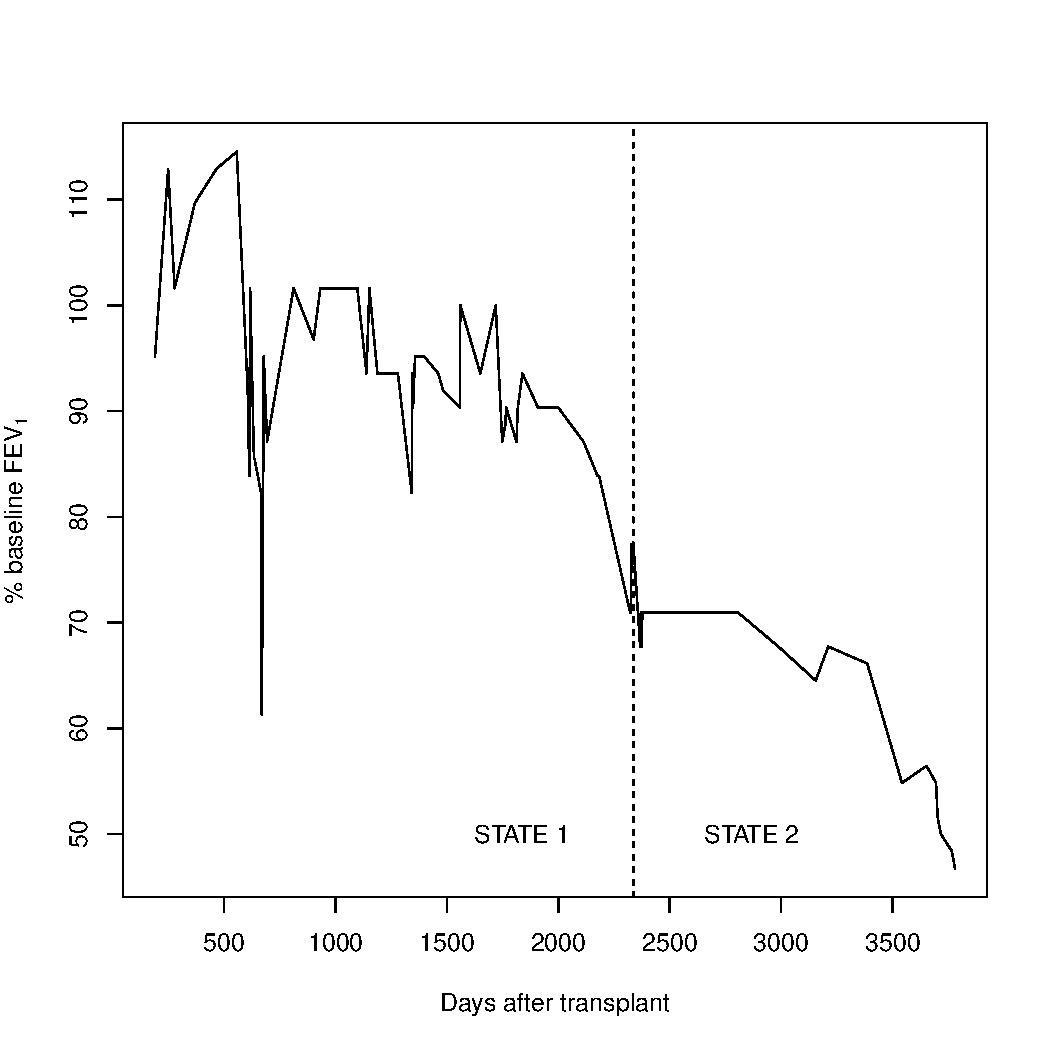
\includegraphics{figures/fev_viterbi}



\paragraph{An alternative way of specifying a misclassification model}

This general framework for specifying hidden Markov models can also be
used to specify multi-state models with misclassification.  A
misclassification model is a hidden Markov model with a categorical
outcome distribution.  So instead of an \Rfunarg{ematrix} argument to
\Rfunction{msm}, we can use a \Rfunarg{hmodel} argument with
\Rfunction{hmmCat} constructor functions.

\Rfunction{hmmCat} takes at least one argument \Rfunarg{prob}, a
vector of probabilities of observing outcomes of $1, 2, \ldots, n$
respectively, where $n$ is the length of \Rfunarg{prob}.  All outcome
probabilities with an initial value of zero are assumed to be fixed at
zero.  \Rfunarg{prob} is scaled if necessary to sum to one.

The model in section \ref{sec:fitting:hmm:misc} specifies that an
individual occupying underlying state 1 can be observed as states 2
(and 1), underlying state 2 can be observed as states 1, 2 or 3, and
state 3 can be observed as states 2 or 3, and underlying state 4
(death) cannot be misclassified. Initial values of 0.1 are given for
the 1-2, 2-1, 2-3 and 3-2 misclassification probabilities.

This is equivalent to the model below, specified using a
\Rfunarg{hmodel} argument to \Rfunction{msm}.  The maximum likelihood
estimates should be the same as before (Model 5).

\begin{Scode}
Qm <- rbind(c(0, 0.148, 0, 0.0171),
            c(0, 0, 0.202, 0.081),
            c(0, 0, 0, 0.126),
            c(0, 0, 0, 0))
cavmisc.msm <- msm(state ~ years, subject = PTNUM, data = cav,
                     hmodel = list (hmmCat(c(0.9, 0.1, 0, 0)),
                                    hmmCat(c(0.1, 0.8, 0.1, 0)),
                                    hmmCat(c(0, 0.1, 0.9, 0)),
                                    hmmIdent(4)),
                     qmatrix = Qm, obstrue=firstobs, deathexact = 4)
cavmisc.msm
\end{Scode}


\subsubsection{Hidden Markov models with multivariate outcomes}

Since version 1.5.2, \Rpackage{msm} can fit models where at each time
point, there are multiple outcomes generated conditionally on a single
hidden Markov state.  The outcomes must be independent conditionally
on the hidden state, but they may be generated from the same or
different univariate distributions.

See \Rfunction{help(hmmMV)} for detailed documentation and a worked
example.



\subsubsection{Defining a new hidden Markov model distribution}

Suppose the hidden Markov model outcome distributions supplied with
\Rpackage{msm} (Table \ref{tab:hmm:dists}) are insufficient.  We want
to define our own univariate distribution, called
\Rfunction{hmmNewDist}, taking two parameters \Robject{location} and
\Robject{scale}.  Download the source package, for example
\texttt{msm-0.7.2.tar.gz} for version 0.7.2, from CRAN and edit the
files in there, as follows.

\begin{enumerate}
\item Add an element to \Robject{.msm.HMODELPARS} in the file
  \texttt{R/constants.R}, naming the parameters of the distribution.
  For example
\begin{Scode}
  newdist = c('location', 'scale')
\end{Scode}

\item Add a corresponding element to the C variable \texttt{HMODELS}
  in the file \texttt{src/lik.c}.  This MUST be in the same position
  as in the \Robject{.msm.HMODELPARS} list.  For example,
\begin{Scode}
hmmfn HMODELS[] = {
  ...,
  hmmNewDist
};.
\end{Scode}

\item The new distribution is allowed to have one parameter which can
  be modelled in terms of covariates.  Add the name of this parameter
  to the named vector \Robject{.msm.LOCPARS} in
  \texttt{R/constants.R}.  For example \texttt{newdist = 'location'}.
  Specify \texttt{newdist = NA} if there is no such parameter.

\item Supposed we have specified a parameter with a non-standard name,
  that is, one which doesn't already appear in
  \Robject{.msm.HMODELPARS}. Standard names include, for example,
  \texttt{'mean'}, \texttt{'sd'}, \texttt{'shape'} or
  \texttt{'scale'}.  Then we should add the allowed range of the
  parameter to \Robject{.msm.PARRANGES}. In this example, we add
  \texttt{meanpars = c(-Inf, Inf)} to \Robject{.msm.PARRANGES}.  This
  ensures that the optimisation to estimate the parameter takes place
  on a suitable scale, for example, a log scale for a parameter
  constrained to be positive.  If the parameter should be fixed during
  maximum likelihood estimation (for example, the denominator of a
  binomial distribution) then add its name to \Robject{.msm.AUXPARS}.

\item Add an R constructor function for the distribution to
  \texttt{R/hmm-dists.R}.  For a simple univariate distribution, this is of the
  form
\begin{Scode}
  hmmNewDist <- function(location, scale)
  {
    hmmDIST(label = "newdist",
    link = "identity",
    r = function(n) rnewdist(n, location, scale),
    match.call())
  }
\end{Scode}

  \begin{itemize}
  \item The \texttt{'label'} must be the same as the name you
    supplied for the new element of \Robject{.msm.HMODELPARS}

  \item \texttt{link} is the link function for modelling the location
    parameter of the distribution as a linear function of covariates. This
    should be the quoted name of an R function.  A log link is
    \texttt{'log'} and a logit link is \texttt{'qlogis'}.  If
    using a new link function other than \texttt{'identity'},
    \texttt{'log'}, or \texttt{'qlogis'}, you should add its name
    to the vector \Robject{.msm.LINKFNS} in \texttt{R/constants.R},
    and add the name of the corresponding inverse link to
    \Robject{.msm.INVLINK}.  You should also add the names of these
    functions to the C array \texttt{LINKFNS} in \texttt{src/lik.c},
    and write the functions if they do not already exist.

  \item \texttt{r} is an R function, of the above format, returning a
    vector of \texttt{n} random values from the distribution.
    You should write this if it doesn't already exist.
  \end{itemize}

\item Add the name of the new constructor function to the NAMESPACE in
  the top-level directory of the source package.

\item Write a C function to compute the probability density of the
  distribution, and put this in \texttt{src/hmm.c}, with a declaration
  in \texttt{src/hmm.h}. This must be of the form
\begin{Scode}
  double hmmNewDist(double x, double *pars)
\end{Scode}

  where \texttt{*pars} is a vector of the parameters of the
  distribution, and the density is evaluated at \texttt{x}.

\item (Optionally) Write a C function to compute the derivatives of
  the probability density with respect to the parameters, and put this
  in \texttt{src/hmmderiv.c}, with a declaration in
  \texttt{src/hmm.h}.  Then add the model to \texttt{DHMODELS} in
  \texttt{lik.c} (in the same position as in \texttt{HMODELS}) and
  \texttt{.msm.HMODELS.DERIV} in \texttt{R/constants.R}.  This will
  generally double the speed of maximum likelihood estimation, but analytic 
  derivatives will not be available for all distributions.
  
\item Update the documentation (\texttt{man/hmm-dists.Rd}) and the
  distribution table in\\ \texttt{inst/doc/msm-manual.Rnw}) if you like.

\item Recompile the package (see the ``Writing R Extensions'' manual)

\end{enumerate}

Your new distribution will be available to use in the \Rfunarg{hmodel}
argument to \Rfunction{msm}, as, for example
\begin{Scode}
hmodel = list(..., hmmNewDist(location = 0, scale = 1), ...)
\end{Scode}
If your distribution may be of interest to others, ask me
(\texttt{chris.jackson@mrc-bsu.cam.ac.uk}) to include it in a future
release.


\clearpage


\message{ !name(msm-manual.Rnw.tex) !offset(-1781) }
